\documentclass{standalone}
\usepackage{preset}
\begin{document}
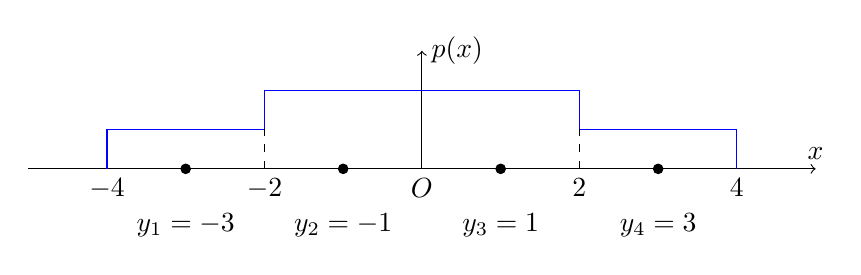
\begin{tikzpicture}[x=10mm,y=60mm]
	\draw[->](-5,0)--(5,0)node[above]{$x$};
	\draw[->](0,0)node[below]{$O$}--(0,.25)node[right]{$p(x)$};
	\foreach \x in {-4,-2,2,4}{
		\draw(\x,0)node[below]{$\x$};
	}
	\foreach \x/\i in{-3/1,-1/2,1/3,3/4}{
		\draw[fill=black](\x,0)ellipse(.06 and .01);
		\draw(\x,-.12)node{$y_\i=\x$};
	}
	\draw[blue](-4,0)--++(0,{1/12})--++(2,0)--++(0,{1/12})--++(4,0)--++(0,{-1/12})--++(2,0)--++(0,{-1/12});
	\draw[dashed](-2,0)--+(0,{1/12});
	\draw[dashed](2,0)--+(0,{1/12});
\end{tikzpicture}
\end{document}
